\documentclass[12pt, a4paper]{article}
\usepackage{amsmath}
\usepackage{amsfonts}
\usepackage{amsthm}
\usepackage{mathtools}
\newtheorem{theorem}{Theorem}[section]
\newtheorem{definition}{Definition}[section]
\numberwithin{equation}{section}
\usepackage{pgfplots}
\pgfplotsset{width=10cm,compat=1.9}
\graphicspath{ {img/} }
\DeclareGraphicsExtensions{.png}

\title{Time series}
\author{Kristian Wichmann}

\begin{document}
\maketitle

\section{Stochastic processes and time series}
\begin{definition}
Let $T$ be a set, called the index set, and $(\Omega, \mathcal{F})$ be a measurable space. Then a stochastic process is a set of probability distributions and associated random variables $\{X_t|t\in T\}$, i.e. $\mathcal{F}$-measurable functions $X_t: \Omega\rightarrow\mathbf{R}$.
\end{definition}

\begin{definition}
For each $\omega\in\Omega^T$ we can define a function $x:T\rightarrow\mathbf{R}$ by:
\begin{equation}
x(t)=x_t=X_t(\omega(t))
\end{equation}
These are known as realizations or sample-paths of the stochastic process.
\end{definition}

\begin{definition}
A stochastic process for which the index set $T\subseteq\mathbf{Z}$ is called a time series.
\end{definition}
As long as there's no chance of confusion, we will use the term 'time series' interchangeably for the stochastic process itself, and any relevant realizations of it.

\section{White noise}
\textit{White noise} is a time series $W_t$ with the following characteristics:
\begin{itemize}
\item The $W_t$'s are pairwise uncorrelated.
\item $E(W_t)=0$
\item The variances for all $W_t$ are equal and finite.
\end{itemize}
We then write $W_t\sim\textrm{wn}(0,\sigma_w^2)$, where $\sigma_w^2$ is the variance.

A slightly stronger criterium, is for the random variables to be i.i.d. In this case we may write $W_t\sim\textrm{iid}(0,\sigma_w^2)$.

Even stronger, the noise may be normally distributed. We then write $W_t\sim \textrm{iid}\ N(0,\sigma_w^2)$.

\subsection{Moving averages of white noise}
In order to smooth out a white noise time series $W_t$, one could average over the values in the immediate vicinity of each $t$. Such a series might be realized as:
\begin{equation}
\label{moving_average}
V_t=\frac{1}{3}(W_{t-1}+W_t+W_{t+1})
\end{equation}
$V_t$ is not a white noise, as the first criterium is no longer satisfied. Such a linear combination of time series data/variables is known as a \textit{filter}.

\subsection{Autoregression}
Imagine two initial values $x_1, x_2$ being given. Then we may form a time series from a white noise $w_t$ as follows:
\begin{equation}
x_t=\alpha x_{t-2}+\beta x_{t-1}+w_t
\end{equation}
Here $\alpha$ and $\beta$ are some constants. This is an example of an \textit{autoregression} - using the last few data points to make predictions about the next one. More about these later.

\section{Random walks}

\subsection{Simple random walk}
Let the random variables $Y_1, Y_2, Y_3,\ldots$ be i.i.d. with the distribution:
\begin{equation}
P(Y_t=1)=1/2,\quad P(Y_t=-1)=1/2
\end{equation}
Now let a time series be defined as:
\begin{equation}
X_0=0,\quad X_t=\sum_{i=1}^t Y_i
\end{equation}
This is known as the \textit{simple random walk}.

\subsubsection{Asymptotic behaviour}
For each of the $Y$'s we have:
\begin{equation}
E[Y_t]=\frac{1}{2}\cdot 1+\frac{1}{2}\cdot(-1)=0,\quad\textrm{var}[Y_t]=\frac{1}{2}1^2+\frac{1}{2}(-1)^2=1
\end{equation}
So, according to the central limit theorem, for large $t$, $X_t$ will be approximately normally distributed:
\begin{equation}
X_t\sim N(0,t),\quad t\gg 1
\end{equation}
This means that the standard deviation for large $t$ is $\sqrt{t}$.

\subsection{Random walk}
Instead of the discrete variables $Y_t$ given above, we might use white noise $W_t\sim\textrm{wn}(0,\sigma_w^2)$. The result is the \textit{random walk} with variance $\sigma_w^2$:
\begin{equation}
X_0=0,\quad X_t=\sum_{i=1}^t W_i
\end{equation}
The second equation could also have been expressed $X_t=X_{t-1}+W_t$.

\subsubsection{Asymptotic behaviour}
Again, we may apply the central limit theorem. For large $t$ we approximately have:
\begin{equation}
X_t\sim N(0,t\sigma_w^2),\quad t\gg 1
\end{equation}
So the standard deviation for large $t$ is $\sqrt{t}\sigma_w$.

\subsection{Random walk with drift}
We now modify the random walk by adding a linear term:
\begin{equation}
X_0=0,\quad X_t=\delta t+\sum_{i=1}^t W_i
\end{equation}
Here $\delta$ is some constant. The second equation could also have been expressed $X_t=\delta+X_{t-1}+W_t$.

\subsubsection{Asymptotic behaviour}
In this case, the central limit theorem gives us
\begin{equation}
X_t\sim N(\delta t,t\sigma_w^2),\quad t\gg 1
\end{equation}
The standard deviation for large $t$ is still $\sqrt{t}\sigma_w$.

\section{Time series descriptors}

Formally, a time series can be described by the family of finite point distribution functions:
\begin{equation}
\label{ts_distribution}
F(c_1,c_2,\ldots,c_n)=P(x_{t_1}\le c_1,x_{t_2}\le c_2,\ldots x_{t_n}\le c_n) 
\end{equation}
Here $t_1, t_2,\ldots,t_n\in T$. While this family does contain all the information about the time series, there's a number of other descriptors that are usually a lot easier easier to compute and/or visualize.

\subsection{The mean function}
For a time series $X_t$, this is simply the series of expectation values:
\begin{equation}
\mu_X(t)=\mu_t=E(X_t)
\end{equation}

\subsubsection{Examples}
The different types of white noise all have a mean function of zero by definition. A moving average is a linear combination of such, so the mean function is still zero. The simple random walk and the random walk are sums of variables with expectation zero, so again we get zero. However, the random walk with drift has a non-zero mean function:
\begin{equation}
\mu(t)=\delta t
\end{equation}

\subsection{The autocovariance function}
For a time series $X_t$, the \textit{autocovariance function} is:
\begin{equation}
\gamma_X(s,t)=\textrm{cov}(X_s,X_t)
\end{equation}
When $s=t$ we get the \textit{variance function} for the series.

Using the definition of covariance, this can be written:
\begin{equation}
\textrm{cov}(X_s,X_t)=E[(X_s-\mu_s)(X_t-\mu_t)]=E[X_s X_t-X_s\mu_t-\mu_s X_t+\mu_s\mu_t)]
\end{equation}
Here $\mu_s=E(X_s), \mu_t=E(X_t)$. Since these are numbers, this is:
\begin{equation}
E(X_s X_t)-E(X_s)\mu_t-\mu_s E(X_t)+\mu_s\mu_t=E(X_s X_t)-\mu_s\mu_t-\mu_s\mu_t+\mu_s\mu_t
\end{equation}
So the autocovariance function can also be calculated as follows:
\begin{equation}
\gamma_X(s,t)=E(X_s X_t)-\mu_s\mu_t
\end{equation}

\subsubsection{Examples}
For the various types of white noise, these are uncorrelated pr. definition when $s\neq t$. When $s=t$ we simply get the variance $\sigma_w^2$. This may be summed up as:
\begin{equation}
\gamma_W(s,t)=\delta_{s,t}\sigma_w^2
\end{equation}

For the moving average, things get a little more interesting. First, when $s=t$:
\begin{equation}
\gamma_V(t,t)=\textrm{cov}\left(\frac{1}{3}(W_{t-1}+W_t+W_{t+1}),\frac{1}{3}(W_{t-1}+W_t+W_{t+1})\right)
\end{equation}
Since the $W$'s are uncorrelated unless the times are equal, this is:
\begin{equation}
\frac{1}{9}(\textrm{cov}(W_{t-1},W_{t-1})+\textrm{cov}(W_t,W_t)+\textrm{cov}(W_{t+1},W_{t+1}))=\frac{1}{3}\sigma_w^2
\end{equation}
When $s=t\pm 1$ we get a similar calculation, but now only two of the terms contribute, so we get $\gamma_V(t\pm 1,t)=\frac{2}{9}\sigma_w^2$. Finally when $s=t\pm 2$ only one term contribute so $\gamma_V(t\pm 2,t)=\frac{1}{9}\sigma_w^2$. Otherwise, the autocorrelation function is zero. Here $\gamma$ only depends on $|s-t|$.

For a simple random walk we have:
\begin{equation}
\gamma_X(s,t)=\textrm{cov}\left(\sum_{i=1}^s Y_i,\sum_{i=1}^t Y_i\right)
\end{equation}
Since the $Y$'s are i.i.d. we only get a contribution at equal times. Hence we get:
\begin{equation}
\gamma_X(s,t)=\min\{s,t\}
\end{equation}

For a random walk, the situation is the same as above, but now each contribution is $\sigma_w^2$, so:
\begin{equation}
\gamma_X(s,t)=\min\{s,t\}\cdot\sigma_w^2
\end{equation}

For a random walk with drift, the added constants do not correlate with the $Y$'s so the result is the same as the case without drift.

\subsection{The autocorrelation function}
It is often convenient to normalize the autocovariance function to get the \textit{autocorrelation function} (or ACF for short):
\begin{equation}
\rho_X(s,t)=\frac{\gamma_X(s,t)}{\sqrt{\gamma_X(s,s)\gamma_X(t,t)}}
\end{equation}
Like ordinary correlations, the autocorrelation function takes on values between -1 and 1.

\subsubsection{Examples}
For white noise, the autocorrelation is zero unless $s=t$. Then we get:
\begin{equation}
\rho_W(t,t)=\frac{\sigma_w^2}{\sqrt{\sigma_w^2\sigma_w^2}}=1
\end{equation}
To sum up $\rho_W(s,t)=\delta_{s,t}$.

For a simple random walk we get:
\begin{equation}
\rho_X(s,t)=\frac{\min\{s,t\}}{\sqrt{st}}
\end{equation}

For a random walk (with or without drift) we get the same result:
\begin{equation}
\rho_X(s,t)=\frac{\min\{s,t\}\cdot\sigma_w^2}{\sqrt{s\sigma_w^2 t\sigma_w^2}}=\frac{\min\{s,t\}}{\sqrt{st}}
\end{equation}

Figure \ref{fig:re_autocorr} graphs $\rho_X$ as a function of $s$ and $t$. Note how is is 1 along the $s=t$ line.

\begin{figure}
\centering
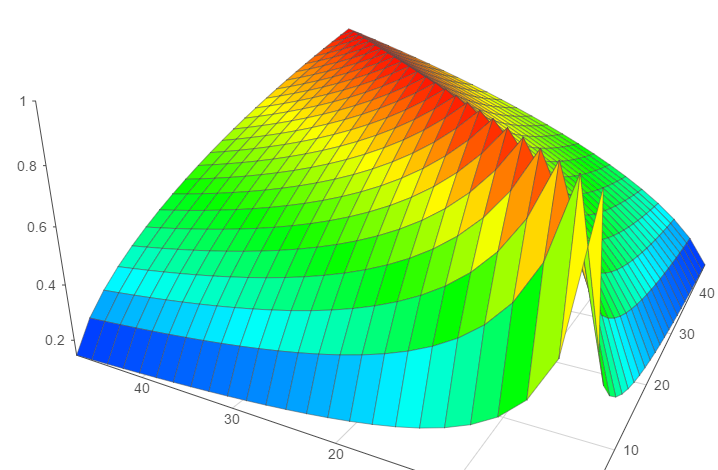
\includegraphics[width=\textwidth]{rw_autocorr}
\caption{The autocorrelation function for a random walk.}
\label{fig:re_autocorr}
\end{figure}

One may wonder what happens to adjacent times:
\begin{equation}
\rho_X(t,t+1)=\frac{t}{\sqrt{t}\sqrt{t+1}}=\sqrt{\frac{t}{t+1}}
\end{equation}
As $t\rightarrow\infty$, this fraction tends to 1. In other words, the adjacent values of a random walk becomes progressively more correlated for large times. Figure \ref{fig:adjacent_times_autocorrelation} graphs this.

\begin{figure}
\centering
\begin{tikzpicture}
\begin{axis}[
    axis lines = left,
    xlabel = $t$,
    ylabel = {Autocorrelation},
    ymin = 0,
    ymax = 1.3,
]
\addplot [
    domain=0:50, 
    samples=50, 
    color=red,
]
{(x/(x+1))^0.5};
\addlegendentry{$\rho_X(t,t+1)$}
\end{axis}
\end{tikzpicture}
\caption{Autocorrelation of adjacent times for random walk.}
\label{fig:adjacent_times_autocorrelation}
\end{figure}

\section{Correlation between time series}
If we have two time series $X_t$ and $Y_t$, we may wish to evaluate if they are correlated in time. Analogously to the last section, we define the \textit{cross-covariance function} as:
\begin{equation}
\gamma_{XY}(s,t)=\textrm{cor}(X_s,Y_t)
\end{equation}
Similarly, the \textit{cross-correlation function} is:
\begin{equation}
\rho_{XY}(s,t)=\frac{\gamma_{XY}(s,t)}{\gamma_X(s,s)\gamma_Y(t,t)}
\end{equation}

\section{Stationarity}

\subsection{Strict stationarity}
A time series $X_t$ with finite variance for all times, is said to be \textit{strictly stationary} if its properties are invariant under time translation in the following sense:
\begin{equation}
\label{strict_stationarity}
P(x_{t_1}\le c_1,x_{t_2}\le c_2,\ldots x_{t_n}\le c_n)=P(x_{t_1+h}\le c_1,x_{t_2+h}\le c_2,\ldots x_{t_n+h}\le c_n)
\end{equation}
This should be true for all times and translations, and any number of points in time $n$.

This is a very strong condition. Specifically, for $n=1$ we get:
\begin{equation}
P(x_s\le c)=P(x_t\le c)
\end{equation}
This means, that the distribution must be the same for all times. Specifically, the mean function $\mu_X$ must be a constant.

For $n=2$ it similarly implies, that the autocovariance - and hence the autocorrelation - can only depend on the different $t-s$.

\subsection{Weak stationarity}
As noted, strict stationarity is very strong. And it is both rare and hard to demonstrate in a model. Therefore, a weaker condition known as \textit{weak stationarity} is useful. A time series $X_t$ is called weakly stationary (or simply stationary) if:
\begin{itemize}
\item It has finite variance at all times.
\item The mean function $\mu_X$ is a constant.
\item The autocovariance function is time translation invariant: $\gamma_X(t,s)=\gamma_X(s+h,t+h)$. In other words a function $\gamma_X(h)=\gamma_X(t,t+h)$ exists.
\end{itemize}

From the last section it is clear, that a strictly stationary time series is also (weakly) stationary. The converse is not generally true.

Because of this, for a stationary time series we may write $\mu_X(t)=\mu$ and $\gamma_X(s,t)=\gamma_X(t-s)$. Therefore, the autocorrelation function can be written:
\begin{equation}
\rho_X(h)=\frac{\gamma_X(t,t+h)}{\sqrt{\gamma_X(t,t)\gamma_x(t+h,t+h)}}=\frac{\gamma_X(h)}{\gamma_X(0)}
\end{equation}

In addition, because of the symmetry of the covariance, we also have:
\begin{align}
\gamma_X(h)=\gamma_X(t,t+h)=&\textrm{cov}(X_t,X_{t+h})=\\
&\textrm{cov}(X_{t+h},X_t)=\gamma_X(t+h,t)=\gamma_X(-h)
\end{align}
This implies, that the autocorrelation function is a function of the absolute value of $h$ only: $\rho_X(h)=\rho_X(|h|)$.

\subsection{Weak dependence}
A stationary time series is said to be \textit{weakly dependent}, if the autocovariance function $\gamma_X(h)$ tends to zero as $h\rightarrow\infty$.

\subsubsection{Examples}
All the types of white noise are clearly stationary. If the white noise is i.i.d., they are also strictly stationary, since equation \ref{strict_stationarity} reduces to a product of distribution functions.

Moving averages are stationary as is evident from the properties derived in previous sections.

Random walks turn out not to be stationary, as correlation is dependent on both times chosen, not just the difference.

\subsection{Joint stationarity}
Two time series $X_t$ and $Y_t$ are said to be \textit{jointly stationary} if they are both stationary and if the cross-covariance function is a function of lag only:
\begin{equation}
\gamma_{XY}(t+h,t)=\gamma_{XY}(h)
\end{equation}
This function satisfies:
\begin{align}
\gamma_{XY}(h)=\gamma_{XY}(t+h,t)=&\textrm{cov}(X_{t+h},Y_t)=\\
&\textrm{cov}(Y_t,X_{t+h})=\gamma_{YX}(t,t+h)=\gamma_{YX}(-h)
\end{align}

We can now define the \textit{cross-correlation function} (or CCF for short):
\begin{equation}
\rho_{XY}(h)=\frac{\gamma_{XY}(h)}{\sqrt{\gamma_X(0)\gamma_Y(0)}}
\end{equation}

\subsubsection{Example}
Let $W_t$ be a white noise time series. Define two new time series as:
\begin{equation}
X_t=W_t+W_{t-1},\qquad Y_t=W_t-W_{t-1}
\end{equation}
First, we need to check that each series is stationary in itself. It is easily seen, that $\gamma_X(t,t)=\gamma_Y(t,t)=2\sigma^2$, $\gamma_X(t+1,t)=\gamma_Y(t+1,t)=\sigma^2$, and $\sigma_Y(t+1,t)=\gamma_Y(t-1,t)=-\sigma^2$ are the only non-zero autocovariance function values. So both are stationary.

What about the cross-covariance function?
\begin{align}
\gamma_{XY}(t,t)=&\textrm{cov}(W_t+W_{t-1},W_t-W_{t_1})\sigma^2-\sigma^2=0\\
\gamma_{XY}(t+1,t)=&\textrm{cov}(W_{t+1}+W_t,W_t-W_{t-1})=\sigma^2\\
\gamma_{XY}(t-1,t)=&\textrm{cov}(W_{t-1}+W_{t-2},W_t-W_{t-1})=-\sigma^2
\end{align}
All other values are zero. Hence, $X_i$ and $Y_i$ are jointly stationary with cross-correlation function:
\begin{equation}
\rho_{XY}(0)=0,\quad\rho_{XY}(\pm 1)=\frac{\pm\sigma^2}{\sqrt{2\sigma^2\cdot 2\sigma^2}}=\pm\frac{1}{2}
\end{equation}


\section{MA(1) time series}
We've seen moving averages before above. The general MA($q$)-model is:
\begin{equation}
X_t=\varepsilon_t+\theta_1\varepsilon_{t-1}+\theta_2\varepsilon_{t-2}+\ldots +\theta_q\varepsilon_{t-q}
\end{equation}
Here $\varepsilon_t$ is white noise with variance $\sigma^2$. We will focus on the case $q=1$:
\begin{equation}
X_t=\varepsilon_t+\theta\varepsilon_{t-1}
\end{equation}

\subsection{Autocovariance and autocorrelation}
We've seen before, that moving averages are stationary, so autocovariance depends only on the time difference $h$. It is clear, that it is zero for $h>q$. For $q=1$, this means there's only two non-zero cases:
\begin{equation}
\gamma_X(0)=\textrm{var}(\varepsilon_t+\theta\varepsilon_{t-1})=\textrm{var}(\varepsilon_t)+\theta^2\textrm{var}(\varepsilon_{t-1})=(1+\theta^2)\sigma^2
\end{equation}
And:
\begin{equation}
\gamma_X(\pm 1)=\textrm{cov}(\varepsilon_t+\theta\varepsilon_{t-1},\varepsilon_{t+1}+\theta\varepsilon_t)=\theta\sigma^2
\end{equation}
The corresponding autocorrelation function is then:
\begin{equation}
\rho_X(h)=
\begin{cases}
1 & \textrm{for }h=0 \\
\frac{\theta}{1+\theta^2} & \textrm{for }h=\pm 1
\end{cases}
\end{equation}


\section{AR(1) time series}
As noted above, an autoregressive model is one, where the values depend linearly on the ones immediately before it, plus some noise. A series depending on the last $n$ values is denoted as AR($n$) for short. Here we will look closer at the case where $n=1$. In other words, the model is:
\begin{equation}
X_t=\rho X_{t-1}+\varepsilon_t
\end{equation}
Again, $\varepsilon_t$ is white noise with variance $\sigma^2$.

\subsection{Autocovariance and autocorrelation for stationary AR(1)}
Let's start by considering the variance of $X_t$:
\begin{equation}
\textrm{var}(X_t)=\textrm{var}(\rho X_{t-1}+\varepsilon_t)=\rho^2\textrm{var}(\rho X_{t-1})+\sigma^2
\end{equation}
Now, let us assume the series to be stationary. The specifically, the variance has to be constant, and therefore $\textrm{var}(X_t)=\textrm{var}(X_{t-1})$. This means:
\begin{equation}
\label{AR1_variance}
\textrm{var}(X_t)=\rho^2\textrm{var}(\rho X_t)+\sigma^2\Leftrightarrow\textrm{var}(X_t)=\frac{\sigma^2}{1-\rho^2}
\end{equation}
This shows some restrictions on $\rho$ if stationarity is required. First of all $\rho=\pm 1$ gives an infinite variance. And for $|\rho|>1$, the variance is negative according to the equation, which is also problematic. So we will assume $|\rho|<1$ in the following. Figures \ref{fig:ar1_95}, \ref{fig:ar1_70} and \ref{fig:ar1_20} show examples of time series with different values of $\rho$ and the same $\sigma^2$. Note that the closer $\rho$ is to 1, the longer it generally takes for the series to cross the time axis.

\begin{figure}
\centering
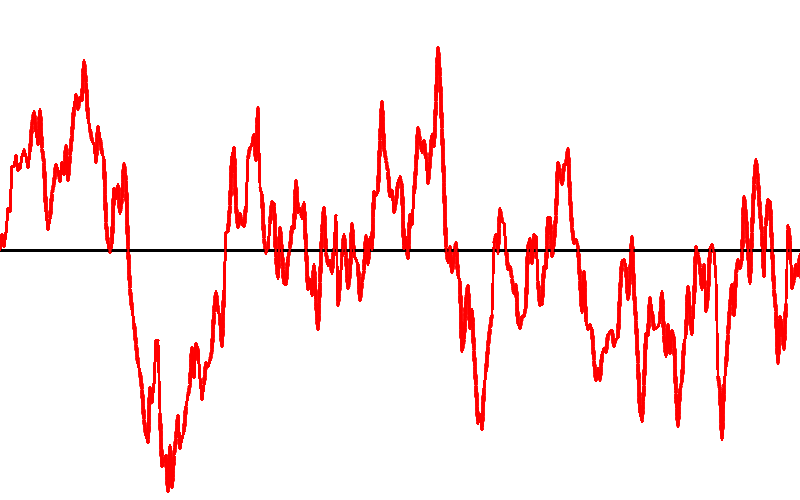
\includegraphics[width=\textwidth]{ar1_95}
\caption{An example of an AR(1) process with $\rho=0.95$.}
\label{fig:ar1_95}
\end{figure}

\begin{figure}
\centering
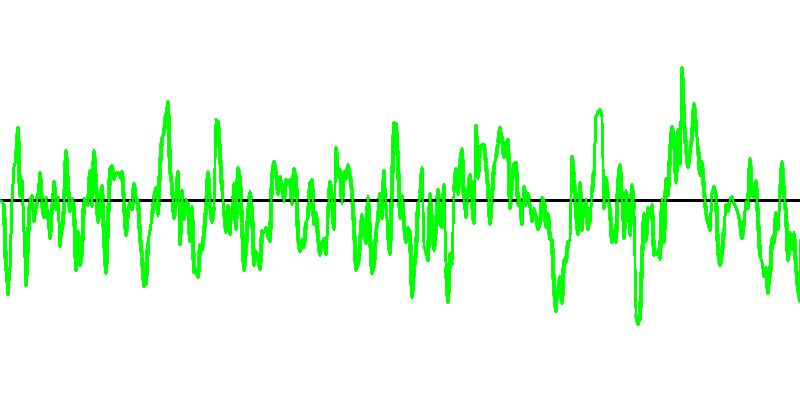
\includegraphics[width=\textwidth]{ar1_70}
\caption{An example of an AR(1) process with $\rho=0.7$.}
\label{fig:ar1_70}
\end{figure}

\begin{figure}
\centering
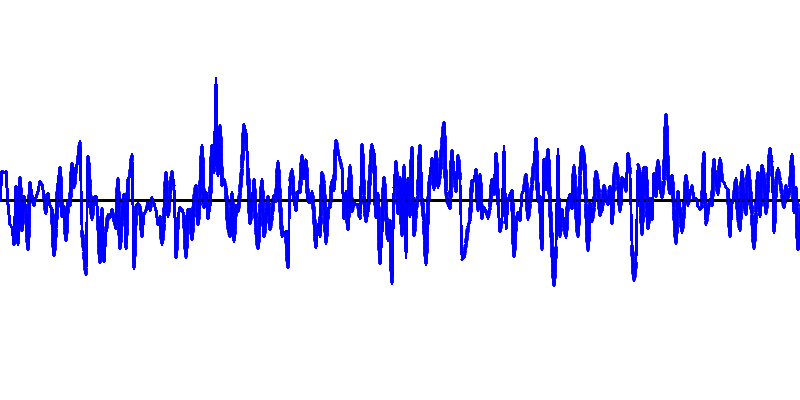
\includegraphics[width=\textwidth]{ar1_20}
\caption{An example of an AR(1) process with $\rho=0.2$.}
\label{fig:ar1_20}
\end{figure}

Now, we turn to the autocovariance function for $h\neq 0$. Let's start with $h=1$. Here we see that:
\begin{equation}
X_t=\rho X_{t-1}+\varepsilon_t=\rho(\rho X_{t-2}+\varepsilon_{t-1})+\varepsilon_t=\rho^2 X_{t-2}+\rho\varepsilon_{t-1}+\varepsilon_t
\end{equation}
In fact, for any $h>0$, we could iterate this substitution process to get:
\begin{equation}
X_t=\rho^h X_{t-h}+\rho^{h-1}\varepsilon_{t-h+1}+\rho^{h-2}\varepsilon_{t-h+2}+\cdots+\varepsilon_t
\end{equation}
Now, it is easy to compute the autocovariance, since only the $X$-term contribute:
\begin{equation}
\gamma_X(h)=\textrm{cov}(X_{t-h},X_t)=\textrm{cov}(X_{t-h},\rho^h X_{t-h})=\rho^h\textrm{var}(X_{t-h})=\rho^h\frac{\sigma^2}{1-\rho^2}
\end{equation}
Here equation \ref{AR1_variance} has been used. This means that the autocorrelation takes on the simple, exponential form:
\begin{equation}
\rho_X(h)=\rho^h
\end{equation}

\section{Lag, backshift and differencing}

\subsection{The lag and backshift operators}
The \textit{lag operator} $L$ for a time series is defined as:
\begin{equation}
LX_t=X_{t-1}
\end{equation}
The lag operator is invertible (at least when the index set is $\mathbb{Z}$):
\begin{equation}
L^{-1}X_t=X_{t+1}
\end{equation}
In general $L$ raised to an arbitrary integer power $n$ is:
\begin{equation}
L^n X_t=X_{t-n}
\end{equation}
The \textit{backshift operator} $B$ is identical to $L$, except for when conditional expectation values are calculated. Let $E_t$ denote the expectation operator based on a realization of the time series up to time $t-1$. The lag operator shifts this realization time, while the backshift operator does not. In other words:
\begin{equation}
L^n E_t[X_{t+j}]=E_{t-n}[X_{t+j-n}],\quad B^n E_t[X_{t+j}]=E_t[X_{t+j-n}]
\end{equation}

\subsection{AR($n$)-models with lag operator}
The general autoregressive model of order $n$ is:
\begin{equation}
X_t=\rho_1 X_{t-1}+\rho_2 X_{t-2}+\ldots+\rho_n X_{t-n}+\varepsilon_t
\end{equation}
This may be rewritten using the lag operator:
\begin{equation}
X_t=\rho_1 L X_t+\rho_2 L^2 X_t+\ldots+\rho_n L^n X_t+\varepsilon_t
\end{equation}
The $X$-dependent part may be written as a \textit{lag polynomial}:
\begin{equation}
X_t=(\rho_1 L+\rho_2 L^2+\ldots+\rho_n L^n)X_t+\varepsilon_t
\end{equation}
Or rearranging:
\begin{equation}
\label{AR_polynomial}
\underbrace{\left(1-\sum_{i=1}^n\theta_i L^i\right)}_{\phi(L)}X_t=\varepsilon_t
\end{equation}
Here, we have introduced $\phi(z)$, the \textit{characteristic polynomial} of the process.

\subsection{Differencing}
When examining a time series, it is often useful to \textit{difference} it. This means calculating (and usually plotting) the series $\Delta X_t=X_t-X_{t-1}$. It is essentially a discrete differentiation. Using the lag operator, this can be written as:
\begin{equation}
\Delta X_t=(1-L)X_t
\end{equation}
Similarly, higher order differings can be defined through:
\begin{equation}
\Delta^d X_t=(1-L)^d X_t
\end{equation}
For $d\ge 1$ all of these are examples of \textit{lag polynomial} operators, since they're expressed as a polynomial form of $L$.

\subsection{I($d$) time series}
A time series of \textit{order of integration} $d$, I($d$), is a series which reduces to white noise after being differenced $d$ times (usually, the lowest of such $n$'s is used). So:
\begin{equation}
\Delta^d X_t=(1-L)^d X_t=\varepsilon_t
\end{equation}
Note the similarity to equation \ref{AR_polynomial}. As an example, an I(1) process is simply a random walk, since:
\begin{equation}
(1-L)X_t=X_t-X_{t-1}=\varepsilon_t\Leftrightarrow X_t=X_{t-1}+\varepsilon_t
\end{equation}
In general, such series are non-stationary.

\section{Markov chains}
A \textit{Markov chain} is a time series, in which the conditional distribution of $X_{n+1}$ given the realizations of $X_0, X_1,\ldots, X_n$ only depends on the realization of $X_n$. Formally:
\begin{equation}
P(X_{n+1}=s|X_0=x_0, X_1=x_1,\ldots, X_n=x_n)=P(X_{n+1}=s|X_n=x_n)
\end{equation}


\subsection{Markov chains with a finite number of states}
In the case where each $X$ only has a finite number of realizations $n$, the Markov chain can be conveniently specified in matrix form. Assume the realization of $X_n$ is state $i$, then we might ask what to probability of $X_{n+1}$ being realized as state $j$. This probability is called $p_{ij}$. These probabilities can be neatly organized in matrix form:
\begin{equation}
A=\begin{pmatrix}
p_{11}	& p_{21}	& \cdots	& p_{n1} \\
p_{12}	& p_{22}	& \cdots	& p_{n2} \\
\vdots	& \vdots	& \ddots	& \vdots \\
p_{1n}	& p_{2n}	& \cdots	& p_{nn}
\end{pmatrix}
\end{equation}
Since the $n$ states exhaust the possibilities, each column must sum to 1:
\begin{equation}
\sum_{j=1}^n p_{ij}=1,\quad i\in{1,2,\ldots n}
\end{equation}

\section{Martingales}

\end{document}